
\documentclass[a4paper,11pt]{article}%,twocolumn
%% packages

\usepackage{blindtext} % needed for creating dummy text passages
%\usepackage{ngerman} % needed for German default language
\usepackage{amsmath} % needed for command eqref
\usepackage{amssymb} % needed for math fonts
\usepackage[colorlinks=true,breaklinks]{hyperref} % needed for creating hyperlinks in the document, the option colorlinks=true gets rid of the awful boxes, breaklinks breaks lonkg links (list of figures), and ngerman sets everything for german as default hyperlinks language
\usepackage[hyphenbreaks]{breakurl} % ben�tigt f�r das Brechen von URLs in Literaturreferenzen, hyphenbreaks auch bei links, die �ber eine Seite gehen (mit hyphenation).
\usepackage{xcolor}
\definecolor{c1}{rgb}{0,0,1} % blue
\definecolor{c2}{rgb}{0,0.3,0.9} % light blue
\definecolor{c3}{rgb}{0.3,0,0.9} % red blue
\hypersetup{
    linkcolor={c1}, % internal links
    citecolor={c2}, % citations
    urlcolor={c3} % external links/urls
}
%\usepackage{cite} % needed for cite
\usepackage[square,authoryear]{natbib} % needed for cite and abbrvnat bibliography style
\usepackage[nottoc]{tocbibind} % needed for displaying bibliography and other in the table of contents
\usepackage{graphicx} % needed for \includegraphics 
\usepackage{longtable} % needed for long tables over pages
\usepackage{bigstrut} % needed for the command \bigstrut
\usepackage{enumerate} % needed for some options in enumerate
%\usepackage{todonotes} % needed for todos
\usepackage{makeidx} % needed for creating an index
\makeindex
\usepackage{gensymb}
\usepackage{url}
\usepackage{psfrag}
\usepackage{multirow}
\usepackage{subfigure}
%% page settings

\usepackage[top=20mm, bottom=20mm,left=15mm,right=15mm]{geometry} % needed for page border settings
\parindent=0mm % for space of first line of new text block
\sloppy % for writing with hyphenless justification (tries to)
\hyphenation{} % use hyphenation of tolerance parametershttp://www.jr-x.de/publikationen/latex/tipps/zeilenumbruch.html
\hyphenpenalty=10000
\exhyphenpenalty=10000
\usepackage{fancyhdr} % needed for head and foot options
%% my macros

%% Text fomats
\newcommand{\tbi}[1]{\textbf{\textit{#1}}}

%% Math fonts
\newcommand{\bbA}{\mathbb{A}}
\newcommand{\bbB}{\mathbb{B}}
\newcommand{\bbC}{\mathbb{C}}
\newcommand{\bbD}{\mathbb{D}}
\newcommand{\bbE}{\mathbb{E}}
\newcommand{\bbF}{\mathbb{F}}
\newcommand{\bbG}{\mathbb{G}}
\newcommand{\bbH}{\mathbb{H}}
\newcommand{\bbI}{\mathbb{I}}
\newcommand{\bbJ}{\mathbb{J}}
\newcommand{\bbK}{\mathbb{K}}
\newcommand{\bbL}{\mathbb{L}}
\newcommand{\bbM}{\mathbb{M}}
\newcommand{\bbN}{\mathbb{N}}
\newcommand{\bbO}{\mathbb{O}}
\newcommand{\bbP}{\mathbb{P}}
\newcommand{\bbQ}{\mathbb{Q}}
\newcommand{\bbR}{\mathbb{R}}
\newcommand{\bbS}{\mathbb{S}}
\newcommand{\bbT}{\mathbb{T}}
\newcommand{\bbU}{\mathbb{U}}
\newcommand{\bbV}{\mathbb{V}}
\newcommand{\bbW}{\mathbb{W}}
\newcommand{\bbX}{\mathbb{X}}
\newcommand{\bbY}{\mathbb{Y}}
\newcommand{\bbZ}{\mathbb{Z}}
\usepackage[ framed, numbered]{matlab-prettifier}%framed,%
\usepackage{listings}
\usepackage{physics}
\usepackage{pdfpages}
\usepackage[toc,page]{appendix}
\usepackage{float}
\usepackage{hyperref}

\newenvironment{qanda}{\setlength{\parindent}{0pt}}{\bigskip}
\newcommand{\Q}{\bigskip\bfseries Q: }
\newcommand{\A}{\par\textbf{Answer: } \normalfont}

\begin{document}
\begin{titlepage}
\center % Center everything on the page

%-------------------------------------------------------------------------------------
%	HEADING SECTIONS
%------------------------------------------------------------------------------------
\textbf{\large Department of Electrical and Computer Engineering}\\[0.5cm]
\textbf{\Large University of Colorado at Boulder}\\[1cm]
\textbf{\large ECEN5623 - Real Time Embedded Systems }\\[2cm]

\includegraphics[width=0.3\textwidth]{figures/cu}\\[2cm]

	
%-------------------------------------------------------------------------------------
%	TITLE SECTION
%------------------------------------------------------------------------------------
\textbf{\Huge Exercise 5 }\\[0.2cm]



%----------------------------------------------------------------------------------------
%	MEMBERS SECTION
%----------------------------------------------------------------------------------------


\vfill

\textbf{\large Submitted by}\\[0.5cm]

{\large Parth | Jithedra}\\[0.5cm]	

%----------------------------------------------------------------------------------------
%	DATE SECTION
%----------------------------------------------------------------------------------------

\textbf{\large Submitted on}
\textbf{\Large \today} % Date, change the \today to a set date if you want to be precise

%----------------------------------------------------------------------------------------

\vfill % Fill the rest of the page with whitespace

\end{titlepage}


\pagebreak

\tableofcontents
\listoffigures
\listoftables
\vfill
\begin{center}
	\textbf{\textit{*PDF is clickable}}
\end{center}

\pagebreak



\begin{qanda}
	\section{Question 1}
	\begin{enumerate}
		\item[] \Q [20 points] The Rate Monotonic Policy states that services which share a CPU core should multiplex it (with context switches that preempt and dispatch tasks) based on priority, where highest priority is assigned to the most frequently requested service and lowest priority is assigned to the least frequently requested AND total shared CPU core utilization must preserve some margin (not be fully utilized or overloaded).
			\begin{enumerate}
				\addcontentsline{toc}{subsection}{A}
				\item \Q Draw a timing diagram for three services S1, S2, and S3 with T1=3, C1=1, T2=5, C2=2, T3=15, C3=3 where all times are in milliseconds. [Note that you can find examples of timing diagrams in Lecture and here and in Canvas – note that we have not yet covered dynamic priorities, just RM fixed policy described here, so ignore EDF and LLF for now].

				\A Rate monotonic scheduling is the hard real time scheduling of choice. This is due to the fact that
				its a static scheduling policy which assigns higher priority for more frequent tasks in a system ,so that
				overall utilization of the system nears 100 percent. Also RM policy shows more deterministic behavior
				during all overload situations .Moreover RM, shows O(1) time complexity while adding new tasks in
				the list . 



	\begin{figure}[H]
		\centering
		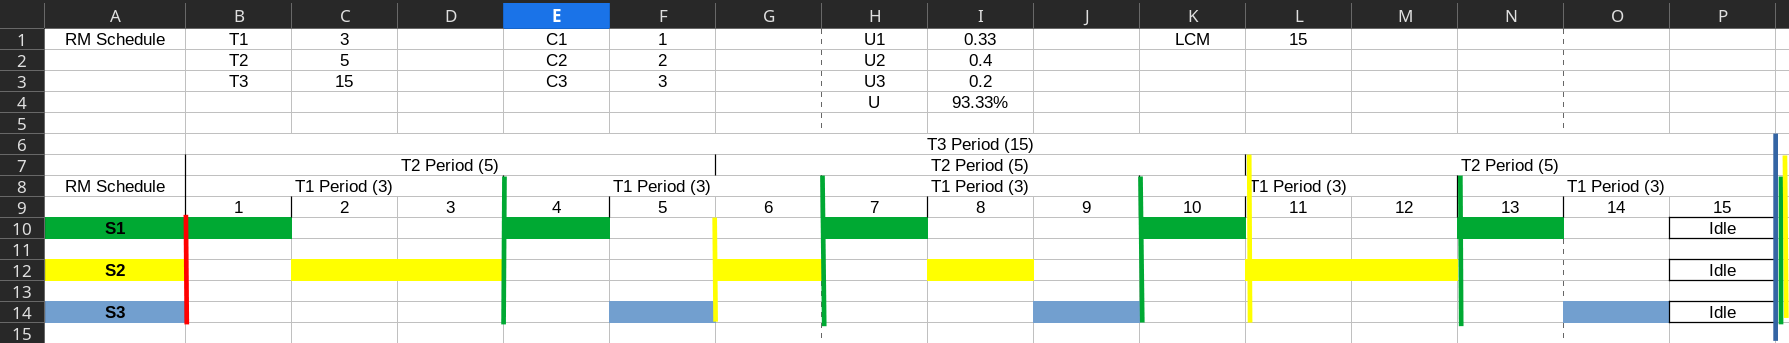
\includegraphics[scale=0.37]{figures/rm.png}
		\caption{Rate monotonic Schedule}
		\label{rm}
	\end{figure}
				      
	\addcontentsline{toc}{subsection}{B}
				\item \Q Label your diagram carefully and describe whether you think the schedule is feasible (mathematically repeatable as an invariant indefinitely) and safe (unlikely to ever miss a deadline).

				      \A \\S1, being the highest priority, runs first at the beginning of every 3 ms interval. \\
					  S2 runs after S1, fitting its execution around the 5 ms mark, respecting its priority over S3 but after S1.\\
					S3, with the lowest priority, fits in where S1 and S2 allow, based on its longer period and lower frequency requirement.\\

				      The schedule is feasible because the total execution time of each service is less than the total period assigned to each service. Secondly, there has been no overlapping in execution times. Thus, this schedule is safe with no missing deadlines and each service completes its execution before its next period begins.
					  \addcontentsline{toc}{subsection}{C}
				\item \Q What is the total CPU utilization by the three services?

				\A   
				\\CPU Utilization by 3 services:\\

				\begin{flalign*}
				&U = \left(\frac{C_1}{T_1} + \frac{C_2}{T_2} + \frac{C_3}{T_3} \right)&&\\
				&U = \left(\frac{1}{3} + \frac{2}{5} + \frac{3}{15} \right)&&\\
				&U = 0.33 + 0.4 + 0.2&&\\
				&U =  93.33&&\\
				&\boxed{U = 93.33\%}&&\\
				\end{flalign*}
				    

				• The CPU Utilization upon calculation is 93.33\%.\\
			\end{enumerate}


	\end{enumerate}




	\section{Question 2}
	\begin{enumerate}
		\item[] \Q [20 points] Read through the Apollo 11 Lunar lander computer overload story as reported in RTECS Notes, based on this NASA account, and the descriptions of the 1201/1202 events described by chief software engineer Margaret Hamilton as recounted by Dylan Matthews. Summarize the story.
			\begin{enumerate}
				\addcontentsline{toc}{subsection}{A}
				\item \Q Summary of the Apollo 11 Lunar Story:

				      \A 
					  The Pathfinder's applications were scheduled by the VxWorks RTOS. Since VxWorks provides pre-emptive priority scheduling of threads, tasks were executed as threads with priorities determined by their relative urgency.\\

				      Apollo Lunar Lander is a special type of computer, Apollo Guidance Computer. It is a digital computer that provides computational and electronic interfaces for guidance, navigation, and control. The first computer was based on the Silicon IC. Installed on the board of the Apollo Command Module and the Lunar Module. This computer utilizes the AGC, a 16-bit word length, and uses special ROM for core rope memory. Astronauts communicated with this AGC using the numeric display and keyboard called DSKY. During the Apollo Mission, AGC terminated the “Error 1201/1202”, which indicated the computer overload. Multiple errors were caused by the Lunar Module’s rendezvous radar left “ON” during the landing. The consequence of leaving the radar “ON” led to the comparatively receiving more data than the computer could handle. The software on AGC was able to prioritize the most critical tasks and ignore lesser important ones, which led to proceeding for a safe landing. This is a testament to the robustness and reliability of the AGC Software. Thanks to the team led by Chief Software Engineer, Margaret Hamilton. The 1201/1202 errors were ultimately caused by the human error. The astronauts forgot to turn the rendezvous radar “OFF”.\\


					  The meteorological data gathering task ran as an infrequent, low priority thread, and used the information bus synchronized with mutual exclusion locks (mutexes). Other higher priority threads took precedence when necessary, including a very high priority bus management task, which also accessed the bus with mutexes. Unfortunately in this case, a long-running communications task, having higher priority than the meteorological task, but lower than the bus management task, prevented it from running.\\
					  
					  Soon, a watchdog timer noticed that the bus management task had not been executed for some time, concluded that something had gone wrong, and ordered a total system reset. (Engineers later confessed that system resets had occurred during pre-flight tests. They put these down to a hardware glitch and returned to focusing on the mission-critical landing software.)\\
				\addcontentsline{toc}{subsection}{B}
				\item \Q What was the root cause of the overload and why did it violate Rate Monotonic policy?

				      \A
				      • Priority inversion is the main root cause of the overload.
				      A low-priority task was given the priority over a high-priority task. This caused a delay in the high-priority task’s execution time. Thus, a violation of the Rate Monotonic Policy was caused as the execution time of high-priority tasks was exceeded than anticipated. Thus, caused an overloading situation.
				\addcontentsline{toc}{subsection}{C}
				\item \Q Now, read Liu and Layland’s paper which describes Rate Monotonic policy and the Least Upper Bound – they derive an equation that advises a margin of approximately 30\% of the total CPU as the number of services sharing a single CPU core increases.

				\A
				      
				\addcontentsline{toc}{subsection}{D}
				\item \Q Plot this Least Upper bound as a function of several services.

				      \A
				      Least Upper Bound defines a safety margin that ensures that the system can handle the worst-case scenario of task execution times or WCET.

	\begin{table}[H]
	\centering

	\begin{tabular}{l c c c c c c c c c c}
		\hline
		\textbf{Number of Services}&\textbf{1}&\textbf{2}&\textbf{3}&\textbf{4}&\textbf{5}&\textbf{6}&\textbf{7}&\textbf{8}&\textbf{9}&\textbf{10}\\\hline
		&&\\
		\textbf{Least Upper Bound (in \%)}&30&45&57&66&73&79&83&87&90&93\\

\hline\hline
	\end{tabular}
	\caption{Least Upper Bound}
	\label{filterspecs}
\end{table}

				      As the LUB \(\%\) increases, the number of services sharing a single-CPU core also increases and so does the load with each increment of the service. However, the system’s safety margin reduces as the latter parameters increases.\\
				      30\% margin suggested by Liu-Layland ensures that the system can in fact handle the worst-case scenarios of task execution times. Thus, preventing the overload situation and ensuring real-time guarantees.

				\addcontentsline{toc}{subsection}{E}
				\item \Q Describe 3 key assumptions they make and document 3 or more aspects of their fixed priority LUB derivation that you don’t understand.

				      \A
					  • The THREE key assumptions they make, are:
					  \begin{enumerate}
						\item
						\begin{enumerate}
							\item There are no precedence constraints between the tasks. Each task can execute independently of each other.
							\item Tasks have Worst-case Execution Time (WCET).
							\item Tasks are periodic and have fixed intervals between their times of beginning.
						\end{enumerate}
						\item The THREE aspects of Fixed Priority Least Upper Bound that were not quite understandable, are:
						\begin{enumerate}
							\item How do they handle tasks with deadlines that are different from their periods? What is the key analysis behind this? They assume that the deadline is the same as the period, but this may not be true for every other case.
							\item How do they account for the context-switching overhead in their LUB equation? The context-switching overhead is not explicitly considered in the equation.
							\item How do they handle the task jitter-variation in the start time of execution of the task? Jitter can affect the response time of a task and may not be accounted for.
						\end{enumerate}
					  \end{enumerate}
				
				\addcontentsline{toc}{subsection}{F}
				\item \Q Would RM analysis have prevented the Apollo 11 1201/1202 errors and potential mission abort? Why or why not?

				      \A     • The RM analysis may or may not have prevented the Apollo 11 1201/1202 errors. To support this, we present two arguments:
					  \begin{enumerate}
						\item RM analysis may not have prevented the errors and mission abort because of the root cause – a Software Overload bug due to the priority inversion problem. Low-priority task was given higher priority instead of the high-priority tasks. The execution time of high-priority was extended more than anticipated and thus, a delay was caused.
						Priority Inversion was the problem that needed to be handled preemptively, and the RM analysis may not have been sufficient to prevent the 1201/1202 errors, and the potential mission abort.
						\item RM analysis can determine whether the system is schedulable or not by analyzing the priorities and the periods. It could have identified the error of overload and thrown out a warning about the possible consequence. By reinforcing RM analysis, it could provide a warning to the scheduler to take corrective measures before the system becomes overloaded. Apollo 1201/1202 errors happened due to an overloaded system, RM analysis could have warned the control team before the overload situation ever took place. However, unfortunately, the priority inversion is not accounted for in the RM Analysis.
					  \end{enumerate} 

			\end{enumerate}


	\end{enumerate}


	

	\section{Question 3}
	\begin{enumerate}
		\item[] \Q  [20 points] Download the RT-Clock code from Canvas and build it on a Jetson board, Raspberry Pi, or Altera DE1- SOC board and execute the code.
    	 
			\begin{enumerate}
				\addcontentsline{toc}{subsection}{1}
				\item \Q Describe what the code is doing and make sure you understand clock\_gettime and how to use it to time code execution print or log timestamps between two points in your code.

				\A 
				The RT-clock code is a simple program demonstrating the usage of POSIX real-time clock for measuring the time of execution of delay loop. Firstly, the program sets up the sleep time for a total of 3 secs and then enters a loop where it requests the specified time to sleep using the function – ‘nanosleep()’. The remaining sleep time is checked, if there is still time remaining, the process goes back to sleep. This particular process is repeated until the requested (expected) sleep time has been successfully met or until the maximum number of sleep calls has been reached. Now, the program calculates the difference between the requested and the actual sleep time and prints the results, at the end.\\

				clock\_gettime() function is used for acquiring the current time in nanoseconds from the POSIX real-time clock. It takes two arguments: clock ID and a pointer to the timespec structure. The clock ID specifies the clock to use and the pointer to the timespec structure is used for storing the current time.
				\addcontentsline{toc}{subsection}{B}
				\item \Q Most RTOS vendors brag about three things: 1 Low Interrupt handler latency, 2 Low Context switch time and 3 Stable timer services where interval timer interrupts, timeouts, and knowledge of relative time has low jitter and drift. Why is each important?

				\A
				\begin{enumerate}
					\item \textbf{Low Interrupt handler Latency:}\\ This is a crucial real-time systems parameter as it allows the system to respond quickly to any external event. A lower interrupt handler latency means the system can begin processing an interrupt as soon as it is received. This is often critical in time-bound systems. 
					\item \textbf{Low Context Switch Time:}\\
					This is important in real-time systems because it allows the system to switch between tasks quickly. A lower context switch time renders to be fruitful for the system as it can switch between the tasks without incurring a large overhead, this helps to ensure that tasks meet their deadlines.
					\item \textbf{Stable Timer Services:}\\
					These are crucial for real-time systems as they provide a predictable and consistent way to measure time. Low jitter and drift ensure that the timer services are working accurately and that they can produce reliable consistent time measurements. 
				\end{enumerate}

				\addcontentsline{toc}{subsection}{C}
				\item \Q Do you believe the accuracy provided by the example RT-Clock code? Why or why not?

				\A
				\begin{enumerate}
					\item The output of code RT-Clock on my system (processor AMD Ryzen 5, with debian base) is,
					\begin{figure}[H]
						\centering
						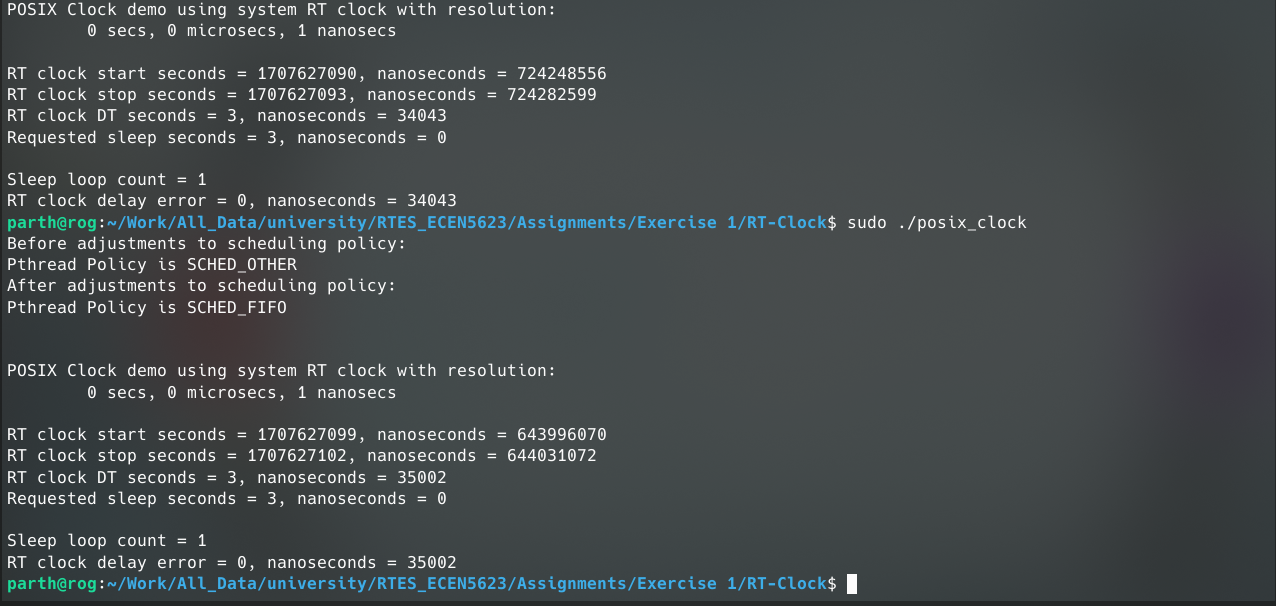
\includegraphics[scale=0.5]{figures/rt_clock_my.png}
						\caption{Rate monotonic OutPut On my linux}
						\label{rmo_on_my_linux}
					\end{figure}
					error was around 34000 - 36000 which is still feasible for some tasks 

					\item The output of the RT\_clock code on Jatson nano is around 202446ns which is much larger than my system, which would not be feasible for some system
					\begin{figure}[H]
						\centering
						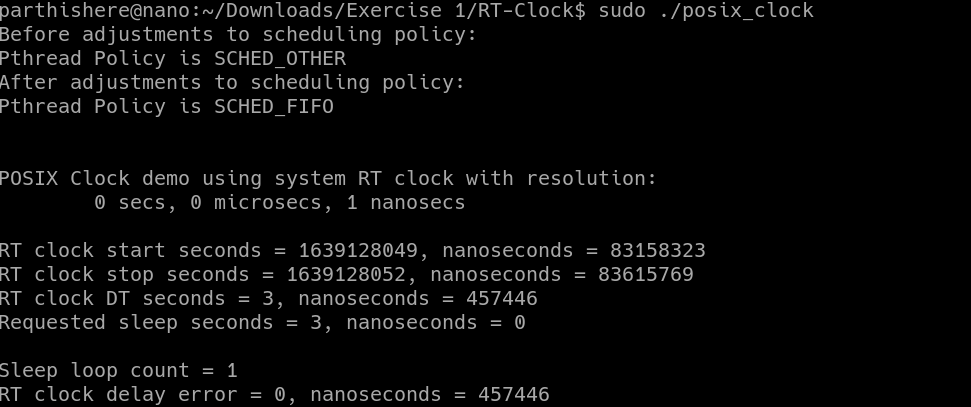
\includegraphics[scale=0.5]{figures/nano.png}
						\caption{Rate monotonic OutPut On Jatson Nano}
						\label{rmo_on_my_linux}
					\end{figure}
					
				\end{enumerate}
				
				The precision of the ‘nanosleep()’ function and the POSIX real-time clock will determine how accurate the RT-Clock code is. POSIX real-time clock is based on the hardware timer and the accuracy is possible on the hardware timer’s precision. The accuracy of the scheduler of the Operating system and the underlying hardware are more factoring parameters that affect the nanosleep() function. This results in the RT-clock code’s accuracy to differ based on the machine it is compiled and run on. Thus, this code sufficiently explains the usage of the necessary functions but should not be deployed in a production setting without testing.\\\\
				Further, the code measures the execution time of the loop using a delay loop and nanosleep() function. There are better and more precise ways to measure time as this may not be the most precise way to do so.\\\\ 
				 Thus, the RT-Clock’s code is not accurate enough for some real-time applications. On top of that, it is necessary to examine and consider the needs of the application and conduct robust testing to ensure the accuracy of the required level is achieved.
			\end{enumerate}
	\end{enumerate}

	\section{Question 4}
	\begin{enumerate}
		\item[] \Q [40 points] This is a challenging problem that requires you to learn a bit about Pthreads in Linux and to implement a schedule that is predictable.
			\begin{enumerate}
				\addcontentsline{toc}{subsection}{A}
				\item \Q          Download, build and run code in the following three example programs: simplethread,
				rt\_simplethread, and rt\_thread\_improved and briefly describe each and output produced. [These example programs can also be found on Canvas] [Note that for real- time scheduling, you must run any SCHED\_FIFO policy threaded application with “sudo” – do man sudo if you don’t know what this is]..

				\A \begin{enumerate}
					\item \textbf{rt\_simple\_thread}
					\begin{enumerate}
						\item Sets up a thread with specific attributes to run with this real-time policy(SCHED\_FIFO). The thread's priority is set just below the maximum to ensure it's treated as a high-priority task. 
						\item The thread does some work: first, it calculates a simple sum for each thread IDs, and then it calculates Fibonacci numbers to simulate a more intensive task.
						\item Prints out information about what the thread did, including how long it took (around 7 milliseconds in this case) and which CPU it ran on (CPU-0, because the program specifies to run on one CPU).
						\item Here are the screenshots of code running with 1 thread and setting threads to 12
						\begin{figure}[H]
							\centering
							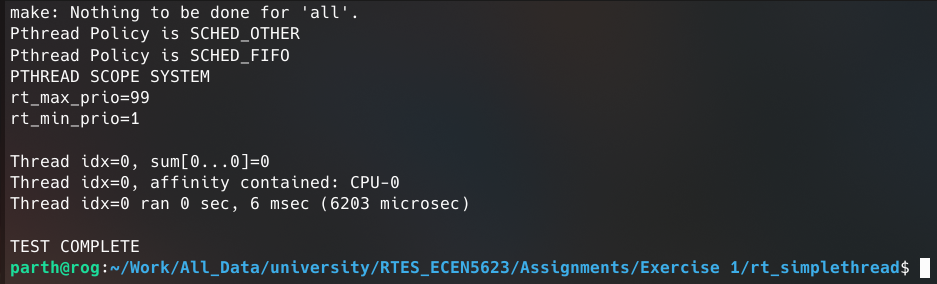
\includegraphics[scale=0.5]{figures/simple_rt_thread.png}
							\caption{Simple RT thread code with one thread}
							\label{rm}
						\end{figure}
						\begin{figure}[H]
							\centering
							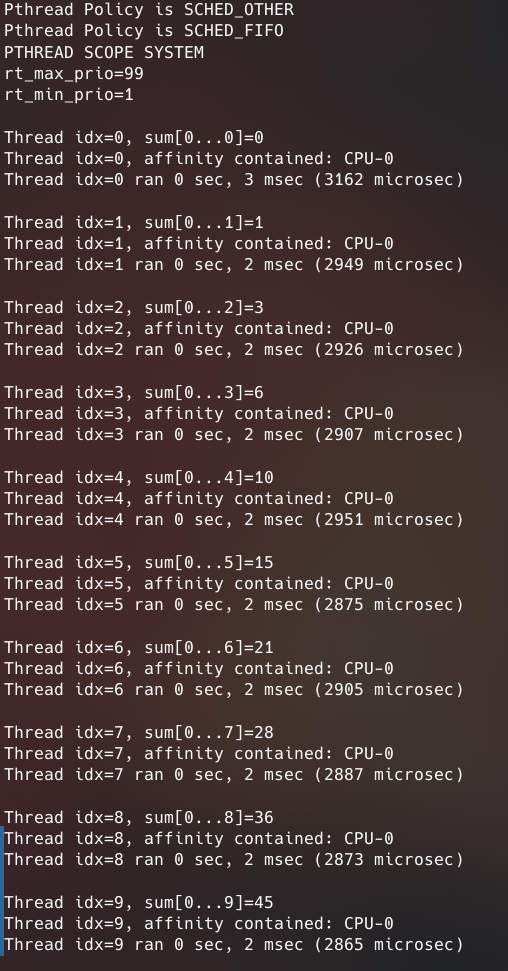
\includegraphics[scale=0.4]{figures/rt_simple12.png}
							\caption{Simple RT thread code with 12 threads}
							\label{rm}
						\end{figure}

						\item \textbf{The output of this code is in the same folder named as rt\_simplethread.txt and rt\_simple12thread.txt (text file) }
						
					\end{enumerate}
					\item \textbf{simplethread}
					\begin{enumerate}
						\item Sets up a thread without any attributes in the main code
						\item The output shows the result of each thread's calculation, that each thread successfully calculates the sum of numbers up to its index. The order of the output might vary between program runs due to the scheduler's decisions on thread execution order. ( we don't have delay in our thread task or our thread task is not that intensive thats why we are getting same order everytime)

						\item Here are the screenshots of output of the code, 
						\begin{figure}[H]
							\centering
							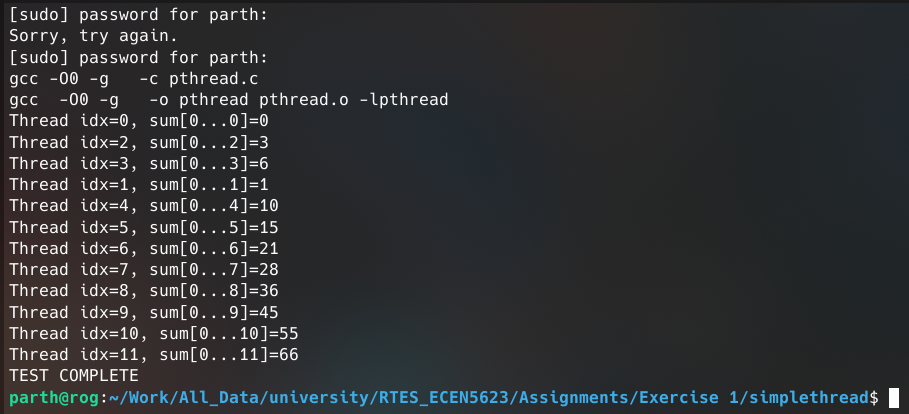
\includegraphics[scale=0.5]{figures/simplethread.png}
							\caption{Simplethread code with 12 threads}
							\label{rm}
						\end{figure}
						

						\item \textbf{The output of this code is in the same folder named as simplethread.txt (text file) }
						
					\end{enumerate}
					\item \textbf{rt\_thread\_improved}
					\begin{enumerate}
						\item It begins by determining the number of processors available and configured on the system, aiming to utilize this information for setting CPU affinity for threads.
						\item CPU Affinity: This code explicitly sets CPU affinity for each thread, ensuring that threads are bound to specific processors. This is a step further in optimizing for real-time performance by reducing the likelihood of CPU cache misses and context switches.
						Number of Processors Utilized: It dynamically checks and utilizes the number of processors available on the system, making it adaptable to run on different hardware configurations.
						\item Prints out information about what the thread did, including how long it took (around 3 milliseconds in this case) and which CPU it ran on
						\item Here are the screenshots of output of the code 
						\begin{figure}[H]
							\centering
							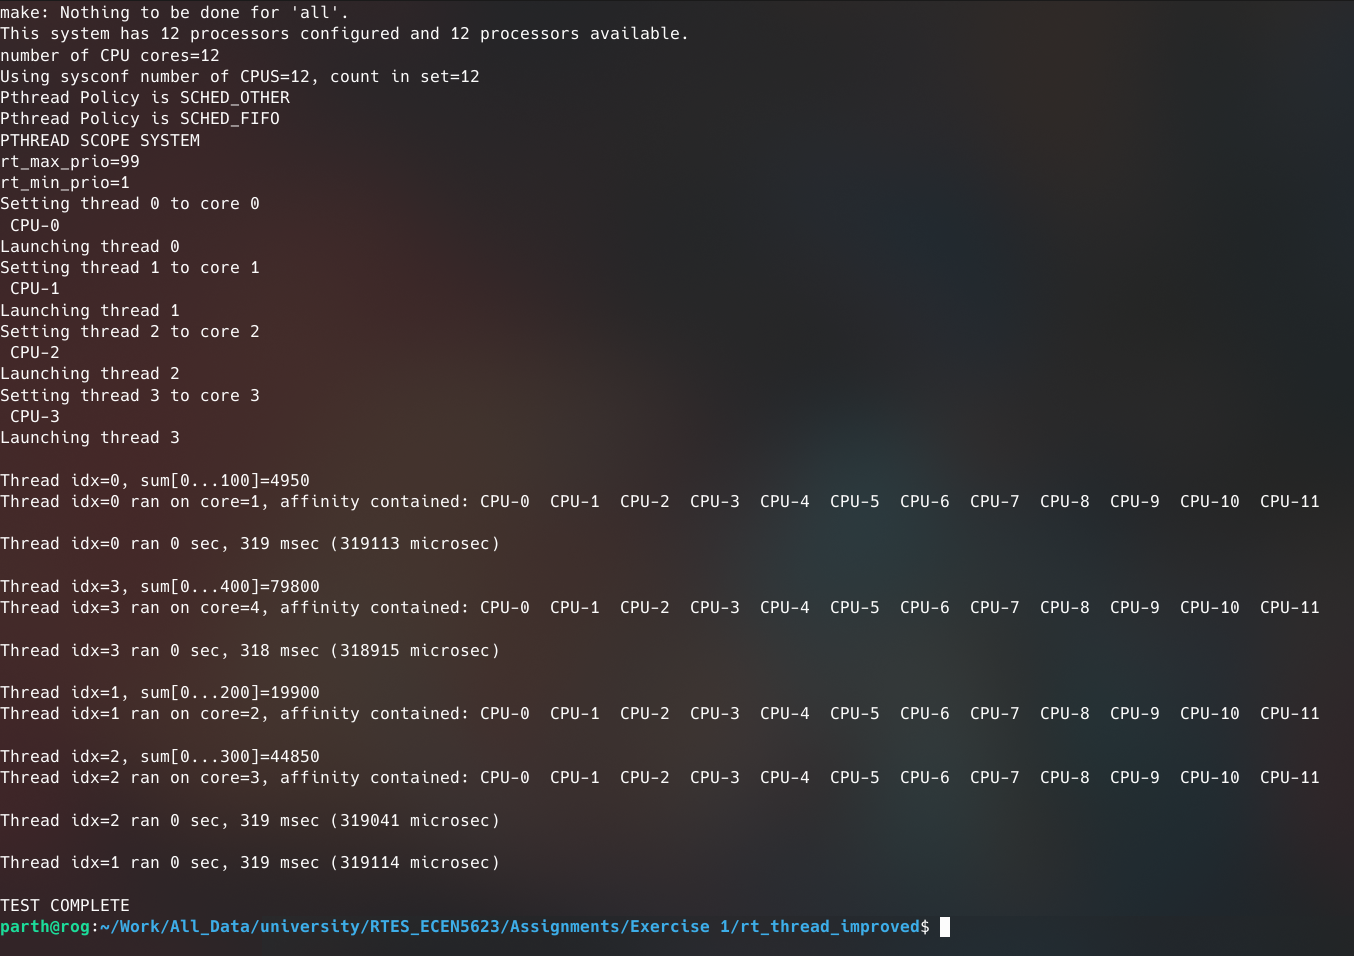
\includegraphics[scale=0.4]{figures/rt_thread_improved.png}
							\caption{RT thread improved with threads running on all cores}
							\label{rm}
						\end{figure}
						

						\item \textbf{The output of this code is in the same folder named as rt\_thread\_improved.txt (text format) }
						
					\end{enumerate}
				\end{enumerate}

				\addcontentsline{toc}{subsection}{B}
				\item \Q Based on the examples for creation of 2 threads provided by incdecthread/pthread.c. Describe the POSIX API functions used by reading POSIX manual pages as needed and commenting your version of this code. Note that this starter example code - testdigest.c is an example that makes use of and sem\_post and sem\_wait and you can use semaphores to synchronize the increment/decrement and other concurrent threading code. Try to make the increment/decrement deterministic (always in the same order). You can make thread execution deterministic two ways – by using SCHED\_FIFO priorities or by using semaphores. Try both and compare methods to make the order deterministic and compare your results.

				      \A \textbf{Summery of the code for semaphore :}
						\begin{enumerate}
							\item gsum: A global variable that both threads will modify.
							\item semaphore: A semaphore used to control access to gsum, ensuring that one thread completes its operation before the other begins.
							\item By using a semaphore with an initial value of 1, the program ensures that only one thread can modify gsum at a time, making the operation order deterministic: first incrementing, then decrementing.
							\item This guarantees that gsum will first be incremented by the sum of numbers from 0 to COUNT-1, and then decremented by the same amount, ending with gsum being 0.
							\item  The output of this code is in the same folder named as output\_sem.txt (text format)
							
						\end{enumerate} 
						\textbf{Summery of the code for making code deterministic by using SCHED\_FIFO :}
						\begin{enumerate}
							\item gsum: A global variable that both threads will modify.
							\item Scheduling and CPU Affinity:\\

							The program attempts to set a real-time scheduling policy (SCHED\_FIFO) for the main process and applies specific priorities to each thread. This policy is a FIFO scheduling algorithm for real-time tasks, where a higher-priority task preempts lower-priority tasks and runs to completion unless it yields, is blocked, or a higher-priority task becomes runnable.\\
							CPU affinity is set for each thread to run on a specific CPU core, aiming to reduce context switching and potentially increase performance predictability.\\
							\item Execution Flow in main:\\
							
							Initializes thread attributes, sets the real-time scheduling policy (SCHED\_FIFO), priorities, and CPU affinity for each thread.\\
							Creates two threads, one for incrementing and the other for decrementing gsum.
							Waits for both threads to complete their execution.
							
							\item This guarantees that gsum will first be incremented by the sum of numbers from 0 to COUNT-1, and then decremented by the same amount
							\item  The output of this code is in the same folder named as output\_sched\_fifo.txt (text format)
							
						\end{enumerate} 
				      
					  \addcontentsline{toc}{subsection}{C}
				\item \Q Describe how you would attempt to implement Linux code to replicate the LCM invariant schedule implemented in the VxWorks RTOS (sequencers/lab1.c) which produces the schedule measured using event analysis shown below:

				\A
				Here's a structured approach to achieve the schedule:
				\begin{enumerate}
					\item 	First, identify the periodic tasks to be scheduled, including their execution periods and computational requirements. For example, if in VxWorks you have tasks running at 10ms and 20ms intervals, you'll replicate this setup.
					\item 	Determine the LCM of all task periods to establish the length of the scheduling cycle. This cycle will repeat indefinitely, and tasks will be scheduled within this framework.
					\item 	For each task, create a POSIX thread (pthread\_t). Threads provide the execution context for each task.
					\item use a real-time scheduling policy (SCHED\_FIFO for priority and first in first out approach) using pthread\_attr\_setschedpolicy() to ensure tasks run according to their priority, which is determined by their periods (Rate Monotonic Scheduling).
					\item  Assign priorities based on the Rate Monotonic principle—shorter periods get higher priorities. Use pthread\_attr\_setschedparam() to set these priorities within the thread attributes.
					\item to improve predictability, bind each thread to a specific CPU core using pthread\_attr\_setaffinity\_np(). 
					\item Semaphore Synchronization:\\
					Initialize semaphores to control the execution start of each task within its period. Semaphores ensure that tasks do not overrun their allocated time and that tasks with longer periods do not start before tasks with shorter periods have completed their execution cycle.

					\item Timing and Execution Loop:
					Each thread should have an execution loop that:
					\begin{enumerate}
						\item Waits on its semaphore at the start of each cycle.
						\item Performs its computational work.
						\item Sleeps or waits for the next cycle based on its period.
					\end{enumerate}
					
					

					\item Task Synchronization for LCM Cycle:
					Create a master control thread or use the main function to synchronize task execution according to the LCM cycle. This involves:
					\begin{enumerate}
						\item Posting to task semaphores at the beginning of each task's period within the LCM cycle.
						\item Monitoring overall cycle time to ensure adherence to the LCM invariant schedule.
					\end{enumerate}
					
					
					
				\end{enumerate}

				
				\addcontentsline{toc}{subsection}{D}
				\item \Q Describe whether you are able to achieve predictable reliable results when you implemented the equivalent code using Linux and pthreads to replicate the LCM invariant schedule. Provide a trace using syslog events and timestamps (Example syslog) and capture your trace to see if it matches VxWorks and the ideal expectation. Explain whether it does and any difference you can note.\\\\
				\A
				\begin{enumerate}
					\item Task Execution and Priority:

					The tasks are assigned priorities inversely proportional to their execution period, adhering to the Rate Monotonic Scheduling (RMS) principle. This is evident from the priorities shown (98 for the 10ms task and 97 for the 20ms task) and their execution order.\\
					The 10ms task (Thread10) runs more frequently than the 20ms task (Thread20), consistent with its shorter period and higher priority.\\\\
					\item Timestamps and Execution Periods:
				
					The timestamps indicate when each task begins execution relative to the start of the test. These timestamps closely align with the expected periodic execution based on each task's period (every 10ms for Thread10 and every 20ms for Thread20), though there's a slight deviation in the arrival times due to the overhead and the precision of timing mechanisms in a general-purpose operating system like Linux.\\
					\item CPU Burst Time:
				
					The burst times recorded are very close to the specified burst times for each task (10ms and 20ms). This suggests that the computational load for each task is being accurately simulated according to the task specifications.

					\item Here are screenshot for the code output
					
					\begin{figure}[H]
						\centering
						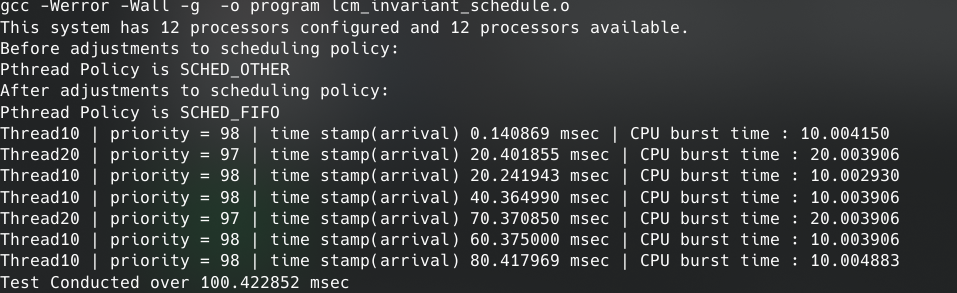
\includegraphics[scale=0.5]{figures/4_e.png}
						\caption{RT thread improved with threads running on all cores}
						\label{rm}
					\end{figure}

					Which shows that the system is feasible and Thread with $C_1 = 10ms$ is getting higher priority than thread with $C_2 = 20ms$, that is why thread running at 20ms is preempting thread running at 50ms

				\end{enumerate} 
				
				
				



			\end{enumerate}


	\end{enumerate}





\end{qanda}




\vfill
\hrule
\vspace{0.5cm}



\vspace{1cm}
\hrule
\vspace{0.5cm}


%---------------------------------------------------------------------------
\end{document}
-
